\documentclass[conference]{IEEEtran}
\IEEEoverridecommandlockouts
% The preceding line is only needed to identify funding in the first footnote. If that is unneeded, please comment it out.
\usepackage{cite}
\usepackage{amsmath,amssymb,amsfonts}
\usepackage{algorithmic}
\usepackage{graphicx}
\usepackage{textcomp}
\usepackage{xcolor}
\def\BibTeX{{\rm B\kern-.05em{\sc i\kern-.025em b}\kern-.08em
    T\kern-.1667em\lower.7ex\hbox{E}\kern-.125emX}}
\begin{document}

\title{Distributed Systems - Surveillance System Project}

\author{\IEEEauthorblockN{1\textsuperscript{st} Cedric Sillaber}
\and
\IEEEauthorblockN{2\textsuperscript{nd} Alan Gallo}
\and
\IEEEauthorblockN{3\textsuperscript{rd} Frantisek Sova}
}
%TODO: explain new async.queue for edge: queue collects data, and asynchronous worker processes it

\maketitle

\section{Introduction}
In our surveillance system, cameras are simulated using the WiseNET dataset. The system is designed to capture video streams and process them efficiently for real-time object and facial recognition. The video data undergoes preprocessing at the edge, minimizing the workload on the cloud, reducing latency, and optimizing the overall performance of the surveillance system. The system leverages edge devices and cloud services to ensure scalability, fast response times, and effective monitoring.  

\section{System architecture}
The video files are stored in camera containers running on a single EC2 instance \ref{fig:architecture}. Each container parses a certain video file into images using OpenCV. These sequences are then sent to edge devices at regular intervals through HTTP, simulating a real-time video stream. Communication between components is handled through a WebSocket, which is capable of managing large payloads and scaling efficiently. Additionally, the EC2 instance houses an alarm container, completing the IoT layer of the system.

\begin{figure}[h!]
    \centering
    %\includegraphics[width=1\linewidth]{res/report/DS_architecture_version2.png}
    \includegraphics[width=1\linewidth]{DS_architecture_version2.png}
    \caption{Example of your architectural diagram.}
    \label{fig:architecture}
\end{figure}

The edge layer consists of a single EC2 instance simulating edge devices in different locations. At the edge, the video data is processed using the YOLO (You Only Look Once) algorithm to detect objects and people. When a person-like object is detected, the relevant data is forwarded to a separate instance in the cloud, ensuring the system can scale dynamically based on demand.

The cloud layer integrates with Amazon Rekognition to perform facial recognition, comparing the detected face against a collection of known individuals. If an unknown person is identified, the cloud server triggers an alert, which is sent back to the edge device and activates the alarm in the IoT layer. This architecture reduces the workload on the cloud, minimizes latency, and ensures the system can handle large volumes of video data in a responsive and efficient manner, making it a robust solution for surveillance applications.



\section{Implementation details}
In our experiment the architecture is as follows.

The IoT layer is represented by 4 camera containers and one alarm container for each edge device. The simulation video comes from set\_3 of WiseNET dataset, which potrays two people appearing in differnt times on the scene. One person can simulate the intruder and the other an employee. 

In order to classifiy intruders, we randomly selected a person and captured several screenshots of the person's face. Those screenshots are uploaded to an AWS Rekognition dataset and used to compare the faces detected by the edge device. The provisioning of the collection and known faces images is done at each start of the cloud server using the boto3 Python package.


While all camera containers will include the whole set of videos, each will select only one based on an environment variable bound to the container. This video is then processed using OpenCV read() function, which returns the sequence of frames. Those are then sent using Socket.IO library to the edge device in an interval simulating the real frame rate. 

The alarm container also connects to the edge server and waits for an event, that will trigger it.

The edge device is an EC2 instance running the YOLO algorithm. The algorithm is implemented in Python and uses the OpenCV library to process the frames. The YOLO algorithm is capable of detecting objects and people in the frames. When a person-like object is detected, the relevant data is sent to the cloud server using a REST API. Images from the IOT layer are received by the edge device using the Socket.IO library. 

In the cloud layer, we implemented a REST API using Python's Flask package to receive images fromc the edge layer. Here, HTTP requests are handled. Those images are directly sent to Rekognition for facial recognition. The result of the image processing is returned in the HTTP response. If an unknown person is detected, an alert is triggered, the edge layer is informed by the HTTP response and the alarm is activated.

Our assumption for the network is that we have several cameras at a location connected to a single edge device. Therefore, the edge device manages multiple cameras, but only one alarm. The cloud layer is assumed to be able to handle multiple edge devices. 
When there is an intruder in one location, the Cloud informs the corresponding edge device to activate the alarm. 

\section{Testing Setup}
In the first weeks of implementing the distributed system, we solely focused on simulating disjoint networks in Docker, utilizing the Docker-Networks feature. 

For every layer, we created a separate Dockerfile.[layer]. A simple \texttt{docker-compose.yaml} file was used to orchestrate the containers. In this orchestration, the camera containers were connected to the edge device, which in turn was connected to the cloud server. 
The IOT containers are connected to the same network as the edge, the edge in addition is connected to the cloud network. 
The following shows the configuration for 

\begin{verbatim}
networks:
  simulation_network:
    driver: bridge
  simulation_network_edge_cloud:
    driver: bridge


# then in the container specification: 
cloud: 
    build:
    context: .
    dockerfile: docker/Dockerfile.cloud
    image: cloud
    networks:
    # subscribe to the network
    - simulation_network_edge_cloud 
\end{verbatim}

This simple setup allowed us to test the communication between the layers and the correct processing of the data. 
Deployment was easy then, just a matter of spinning up the containers on the EC2 instances and adapting the IP addresses in the config file.

\section{Deployment Setup}
The entire distributed system runs on three AWS EC2 instances:

The IoT layer components (4 camera containers and 1 alarm container) are consolidated on a single t2.micro instance, which is sufficient for simulating the video streams and alarm functionality.

The edge layer operates on a t2.medium instance. This increased computational capacity is necessary due to the resource demands of the YOLO algorithm for real-time person detection.

The cloud layer, hosting the AWS Rekognition integration and REST API, runs on a t2.micro instance, as the facial recognition processing is offloaded to AWS services.

This deployment configuration provides a cost-effective setup while ensuring adequate processing power where needed, particularly for the computationally intensive edge layer operations.

\begin{figure}[h!]
    \centering
    %\includegraphics[width=1\linewidth]{res/report/DS_architecture_version2.png}
    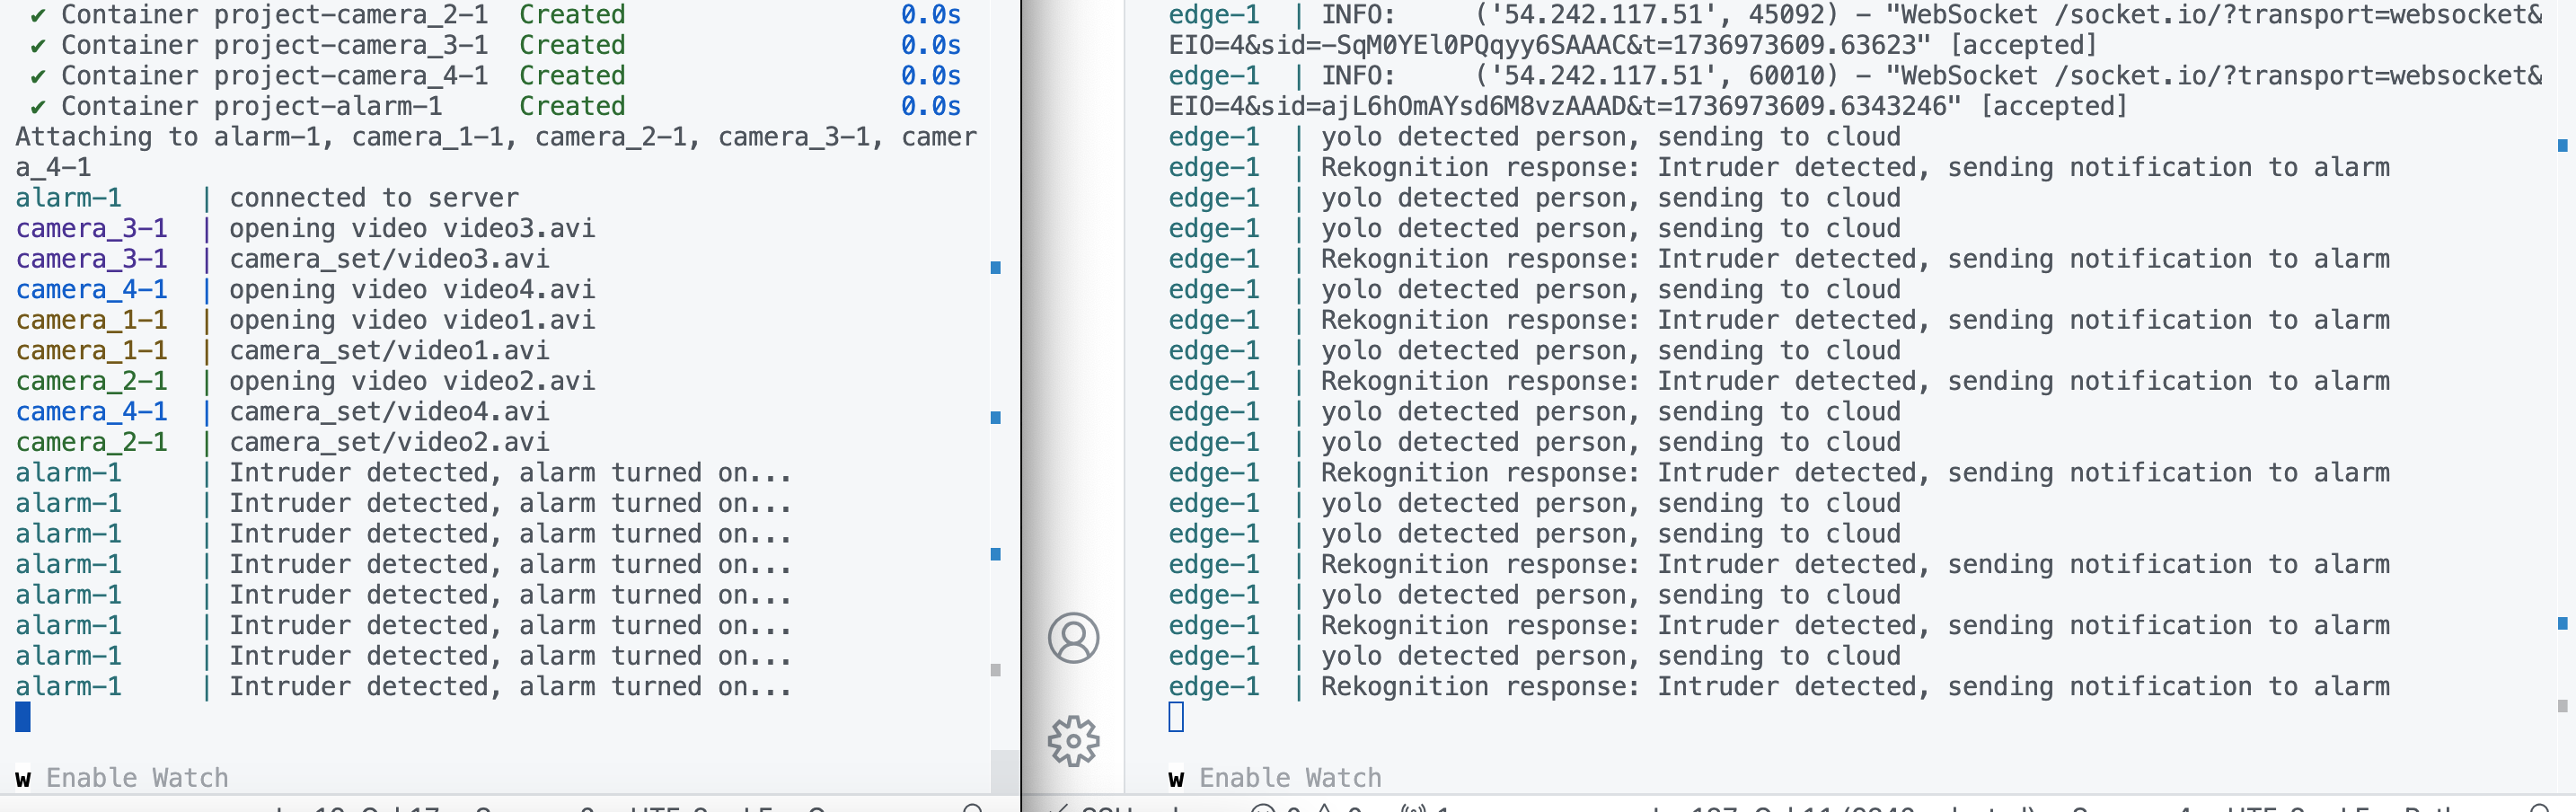
\includegraphics[width=1\linewidth]{deployment2.png}
    \caption{Sucessful detection of intruders.}
    \label{fig:deployment}
\end{figure}
\section{Evaluation}
Evaluation of the response time and scalability (number of devices and traffic) to prove the correctness of your implementation. The more detailed the better. 

\end{document}
